\section{Auswertung}
\label{sec:evaluation}
In diesem Abschnitt wird die Lebensdauer komischer Myonen aus den Messdaten gewonnen.
Um dieses Ziel zu erreichen, ist es erforderlich die Messapparatur zu kalbibrieren.
Alle Fehler werden im Folgenden mit Hilfe
des \texttt{python}-Paktes \texttt{uncertainties} \cite{uncertain} berechnet, welches eine automatische
Gauß'sche Fehlerfortpflanzung bereitstellt.

\subsection{Kalibrierung der Messapparatur}
\label{subsec:calibration}
Die Daten über die Lebensdauer wird mit Hilfe eines Vielkanalanalysators (VKA) gewonnen.
Der VKA teilt die gemessenen Lebensdauern in \num{512} Kanäle (Bins) eines Histogrammes ein.
Dabei ist zu berücksichtigen, das der Zusammenghang zwischen gemessener Lebensdauer und
Kanal linear zusammenhängt.

\noindent Somit ist es Sinnvoll dieses Zusammenhang über eine lineare Funktion

\begin{equation}
f(c) = Ac + B
\end{equation}

\noindent anzunehmen.

\begin{figure}[h!]
	\centering
	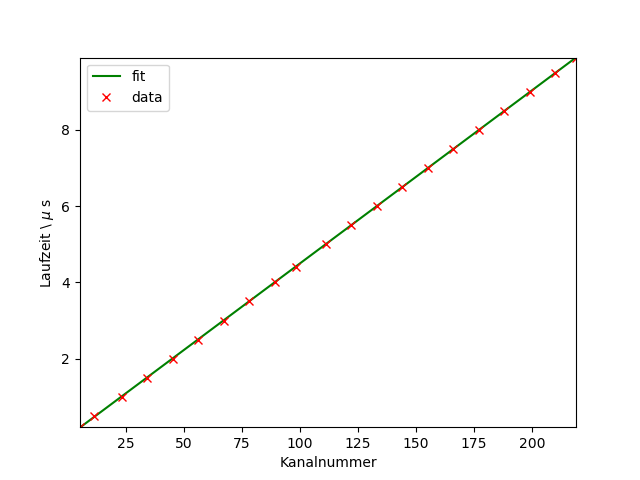
\includegraphics[width=\textwidth]{img/calib.png}
	\caption{Lineare Ausgleichsrechnung zur bestimmung der proportionalität zwischen Kanälen und Zeit}
	\label{abb:cal}
\end{figure}

\noindent Die Ausgleichsrechnung in \ref{abb:cal} liefert somit

\begin{equation}
	t(c) = (0,0454 \pm 0,00003)\frac{\si{\micro\second}}{\text{Kanal}} - (0,035 \pm 0.004) \si{\micro\second}
\end{equation}

\noindent Im der weiteren Auswertung ist lediglich der Prameter $A$ von Interesse, da dieser den die Wartezeit pro Kanal beschreibt und somit den Zusammenhang zwischen VKA Kanal und Wartezeit liefert. Sollten mehrere 
Kanäle im VKA gefüllt worden sein, wurde über die betroffenen Kanalnummern gemittelt.

\subsection{Zeitauflösung der Messapparatur}
\label{subsec:timeresolution}
Um verschiedene Signallaufzeiten zwischen den SEV's und der Koinzidenz ausgleichen zu können, werden Verzögerungsleitungen benutzt, um weitere Verzögerungen in das System einbringen zu können. Durch Messung der Myonen-Zählrate unter Variation der Verzögerungszeiten lässt sich die Auflösungszeit $\Delta t_\text{K}$ der Koinzidenzschaltung als Breite einer Gaußglocke bestimmen.


\subsection{Untergrundrate}
\label{subsec:underground}

Um die Untergrundrate $N_\text{B}$ abschätzen zu können, wird die Wahrscheinlichkeit betrachtet, mit der ein Myon im Tank bei gestarteter Messung in einem Zeitintervall von $T_\text{S} = \SI{10}{\micro \second}$ ein Stopp-Signal erzeugt. Unter der Annahme dass das Auftreten von Myonen normalverteilt ist, lässt sich die Wahrscheinlichkeit $p_i$ einer Messung von $i$ Myonen durch eine Poissonverteilung abschätzen:

\begin{equation}
p_i = \frac{\lambda^i}{i!}\mathrm{e}^{-\lambda}\,,
\end{equation}

\noindent wobei der Erwarungswert der Messung eines Myons mit $\lambda$ bezeichnet wird. Dieser Erwarungswert wird mit der Myonenzählrate identifiziert. Somit liefert die Poissonverteilung die Wahrscheinlichkeit
für die Messung eines Myons.

\noindent Zur Berechnung der Untergrundrate ist es notwendig, die durchschnittliche Anzahl an Myonen zu bestimmen, die in einer Sekunde den Tank passieren.
Die durchgeführte Messung liefert $N_{\text{Start}} = 1426728$ und $t_{\text{Messung}} = 513670 \, \si{\second}$

\begin{equation}
f = \frac{N_{\text{Start}}}{t_{\text{Messung}}} = 2,28 \, \frac{\text{myonen}}{\text{s}}
\end{equation}

\noindent Die Wahrscheinlichkeit, dass genau ein weiteres Myon innerhalb der Suchzeit den Tank durchquert berechnet sich gemäß

\begin{equation}
P = \frac{(T_s \cdot f)^k}{k!} \exp{f \cdot T_s} = 0,00002 \%\,,
\end{equation}


\noindent wobei k = 1 gilt.

\noindent Somit ergeben sich bezogen auf die Startimpulse

\begin{equation}
N_{Err} = 32.53
\end{equation}

\noindent Fehlmessungen. Werden jetzt noch die einzelnen Kanäle berücksichtigt ergibt sich folgende Untergrundrate pro Kanal:

\begin{equation}
U_{\text{B}} = 0,07 \, \frac{\text{Counts}}{\text{Kanal}}\,.
\end{equation}

\subsection{Bestimmung der Lebensdauer}
\label{subsec:lifetime}
Zur bestimmung der Individuallebensdauer der Myonen werden in Abbildung 3 die Daten logarithmiert und an das Ergebnis eine Funktion gemäß

\begin{equation}
f(x) = Ax + U_{\text{B}}
\end{equation}

\noindent gefittet, wobei $U_{\text{B}}$ die Untergrundrate ist.

\begin{figure}[h!]
	\centering
	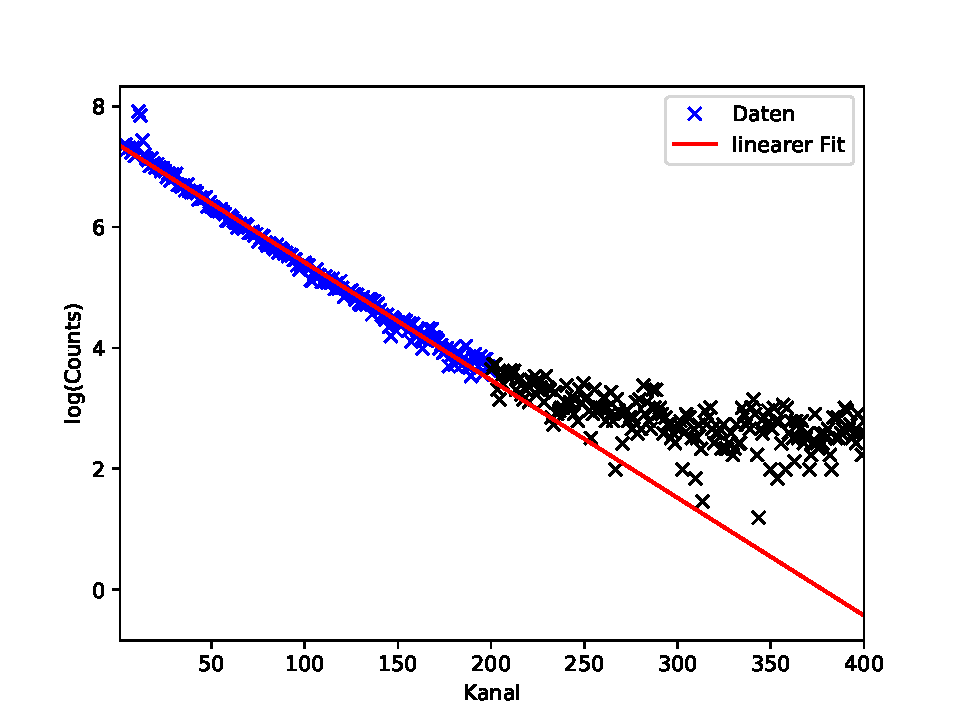
\includegraphics[width=\textwidth]{img/myons.pdf}
	\caption{lineare Ausgleichsrechnung zur bestimmung der Zerfallskonstante}
	\label{abb:fit}
\end{figure}

\begin{table}[h!]
  \centering
\begin{tabular}{cc} \toprule
A   & B  \\ \midrule
10,0192 $\pm$ 0.0001 & 7.33 $\pm$ 0.01 \\
\bottomrule
\label{tab:Fit}
\end{tabular}
\caption{Ergebnisse für die Koeffizienten A und B der Ausgleichsrechnung}
\end{table}

Anschließend wird ein Koeffizientenvergleich unter Berücksichtigung des logarithmierten Zerfallsgesetzes

\begin{equation}
\ln(N(t)) = -\lambda t + \ln{N_0}
\label{eq:LogDecayLaw}
\end{equation}

\noindent durchgeführt. Hieraus folgt für die Zerfallskonstante unter Berücksichtigung der Ergebnisse der Ausgleichsrechnung \ref{tab:Fit} und \ref{eq:LogDecayLaw}

\begin{equation}
\lambda = \frac{1}{\tau} = (0,0191 \pm 0,0001) \,\, \textbackslash \,\, \frac{1}{\text{Kanal}}\,,
\end{equation}

\noindent wobei an dieser Stelle berücksichtigt werden muss, das gemäß \ref{subsec:calibration} ein Zusammenhang zwischen Kanal und Wartezeit besteht. Somit kann
die Lebensdauer durch Sekunden anstatt Kanäle ausgedrückt werden, woraus

\begin{equation}
\tau = \frac{(0,0454 \pm 0,00003) \frac{\si{\micro\second}}{\text{Kanal}}}{\lambda} = (2,330 \pm 0,002) \, \si{\micro\second}
\end{equation}

\noindent folgt. Es ist zu beachten, das die reziproke Zerfallskonstante mit der Wartezeit pro Kanal aus \ref{subsec:calibration} multipliziert wurde.
